\vspace{2mm}
\ffigbox[\FBwidth]{%
\caption{\centering Cas pathologique}\label{fig:dm1_ex05_f1}
}{
    \fbox{
        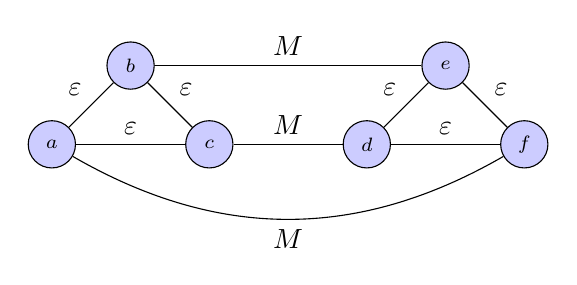
\begin{tikzpicture}[scale=1, main node/.style={circle, draw, fill=blue!20, inner sep=1pt, font=\scriptsize, minimum size=6mm, text=black}]
            % les sommets initiaux
            \node[main node] (1) at (0,0) {\(a\)};
            \node[main node] (2) at (1,1) {\(b\)};
            \node[main node] (3) at (2,0) {\(c\)};
            
            \node[main node] (4) at (4,0) {\(d\)};
            \node[main node] (5) at (5,1) {\(e\)};
            \node[main node] (6) at (6,0) {\(f\)};

            % aretes
            \draw (1) to node[above left] {\(\varepsilon\)} (2);
            \draw (1) to node[above] {\(\varepsilon\)} (3);
            \draw (2) to node[above right] {\(\varepsilon\)} (3);

            \draw (4) to node[above left] {\(\varepsilon\)} (5);
            \draw (4) to node[above] {\(\varepsilon\)} (6);
            \draw (5) to node[above right] {\(\varepsilon\)} (6);

            \draw (2) to node[above] {\(M\)} (5);
            \draw (3) to node[above] {\(M\)} (4);
            
            \draw[bend right] (1) to node[below] {\(M\)} (6);

        \end{tikzpicture}
    }
}